\chapter{AeroShield}

\section{Hardware}


\subsection{Popis súčiastok}

Tu ešte pridám krátke žvásty

\subsubsection{Znižovanie napätia}

Na správne napájanie akčného člena, motorčeka, potrebujeme napätie v rozmedzí 0-3,7V. Na shield je však privázdané pomocou koaxiálneho napájacieho konektora napätie 12V ktoré by motor v priebehu chvíle zničilo. Potrebujeme preto spôsob ako znížiť privádzané napätie, no súčastne neznížiť privádzaný prúd potrebný na pohon motorčeka. Na tieto účely slúži takzvaný buck converter alebo konvertor na zníženie napätia. Hlavnou Časťou konvertora je čip TPS56339 od výrobcu Texas Instruments obr.\ref{OBRAZOK 2.1}.b.

 Na čip je privádzané napätie 12V ktoré sa pomocou zapojenia, vididelného na schéme obr.\ref{OBRAZOK 2.1}.a, znižuje na napätie 3,7V s možnosťou poskytovania prúdu do 3A. Napájanie motora musí byť realizované externe pomocou koaxiálneho napájacieho konektora, z dôvodu vysokého prúdu odoberaného motorom počas vysokého zaťaženia. Rovnaký konektor sa síce nachádza aj na doske Arduino UNO a pomocou VIN pinu sa dajú napájať napätím 0-12V aj iné zariadenia, avšak tento pin je napojený na diódu obmedzujúcu prúd na 1A\cite{ampere}\cite{ampere2}.

\begin{figure}[!tbh]
\hfill
\subfigure[Schéma zapojenia konvertora napätia.]{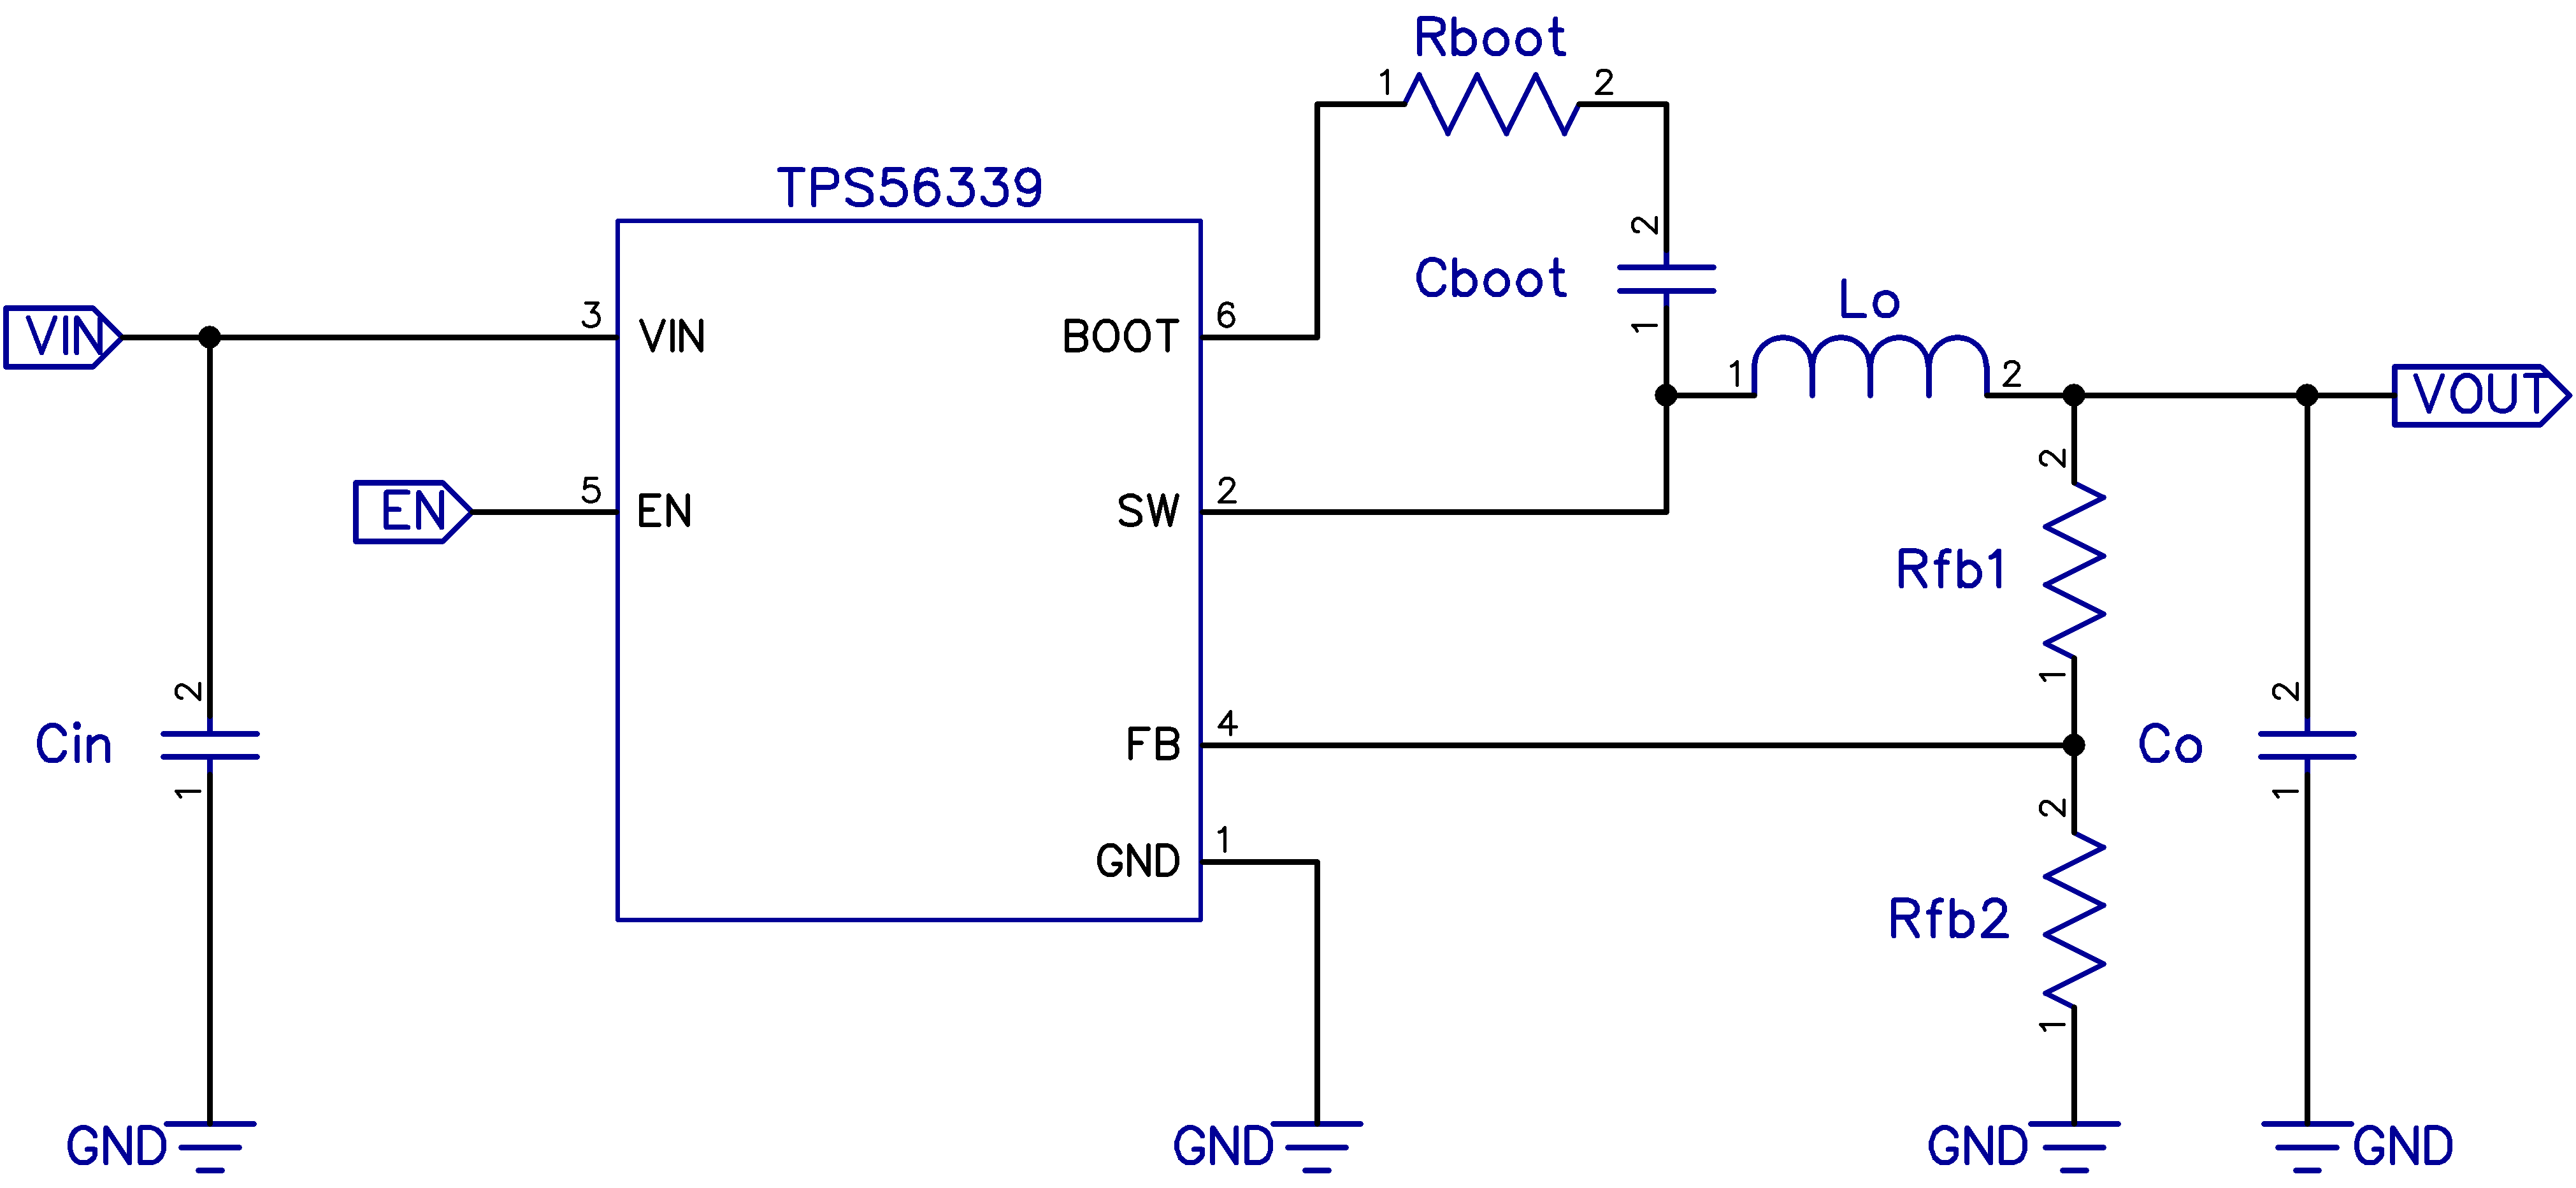
\includegraphics[width=9cm]{obr/schemaBuck.png}}
\hfill
\subfigure[{čip TPS56339\cite{buckobr}}]{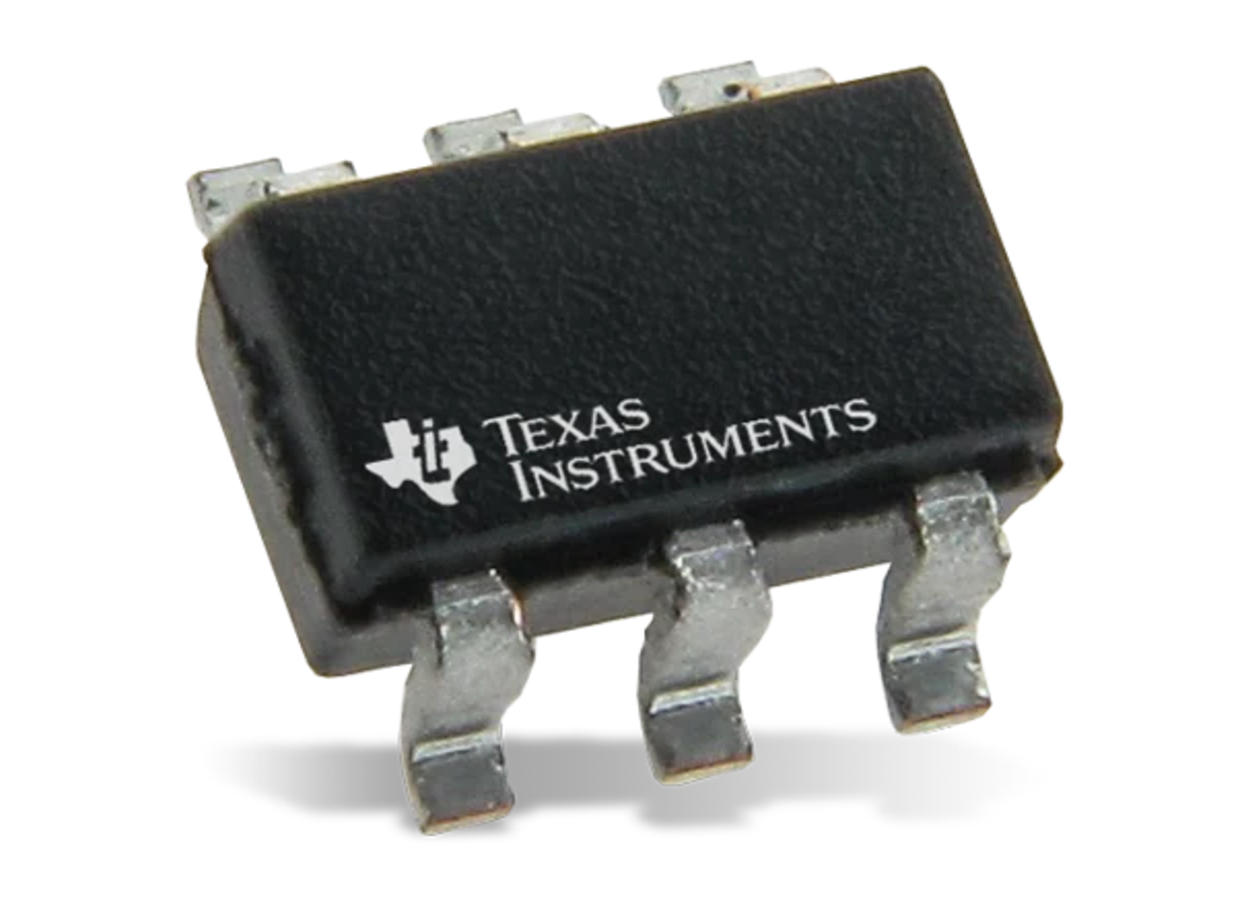
\includegraphics[width=5cm]{obr/cip.eps}}
\hfill
\caption{buck converter}\label{OBRAZOK 2.1}
\end{figure}


\subsubsection{motor}

akc clen motor hovor bam!
neviem aky mam motor :(
poriesime

PWM a mosfet spomeň

\vspace{4cm}

\subsubsection{meranie prúdu}

Pre čo najpresnejšie ovládanie akčného člena sústavy, motora, je dobré vedieť nie len napätie, ktorým je motor ovládaný, ale aj prúd, ktorý motor odoberá. Na tieto účely sa používajú monitory prúdu, takzvané ("current shunt monitors"). V AeroShielde je použitý snímač INA169NA/250 od výrobcu Texas Instruments obr.\ref{OBRAZOK 2.3}.b.

INA169 je "high-side current monitor", čo znamená, že na kladnú stranu je umiestnený špeciálny rezistor ("shunt resistor") a INA169 meria úbytok napätia na tomto rezistore obr.\ref{OBRAZOK 2.3}.a. Na základe nameraného úbytku napätia vysiela senzor určité napätie ktoré sa následne znásobuje a toto napätie môžeme zaznamenávať. Pomocou základnej matematiky udáva výstupné napätie prúd pretekajúci cez shunt rezistor\cite{INA}.

\begin{figure}[!tbh]
\hfill
\subfigure[Schéma zapojenia snímača prúdu.]{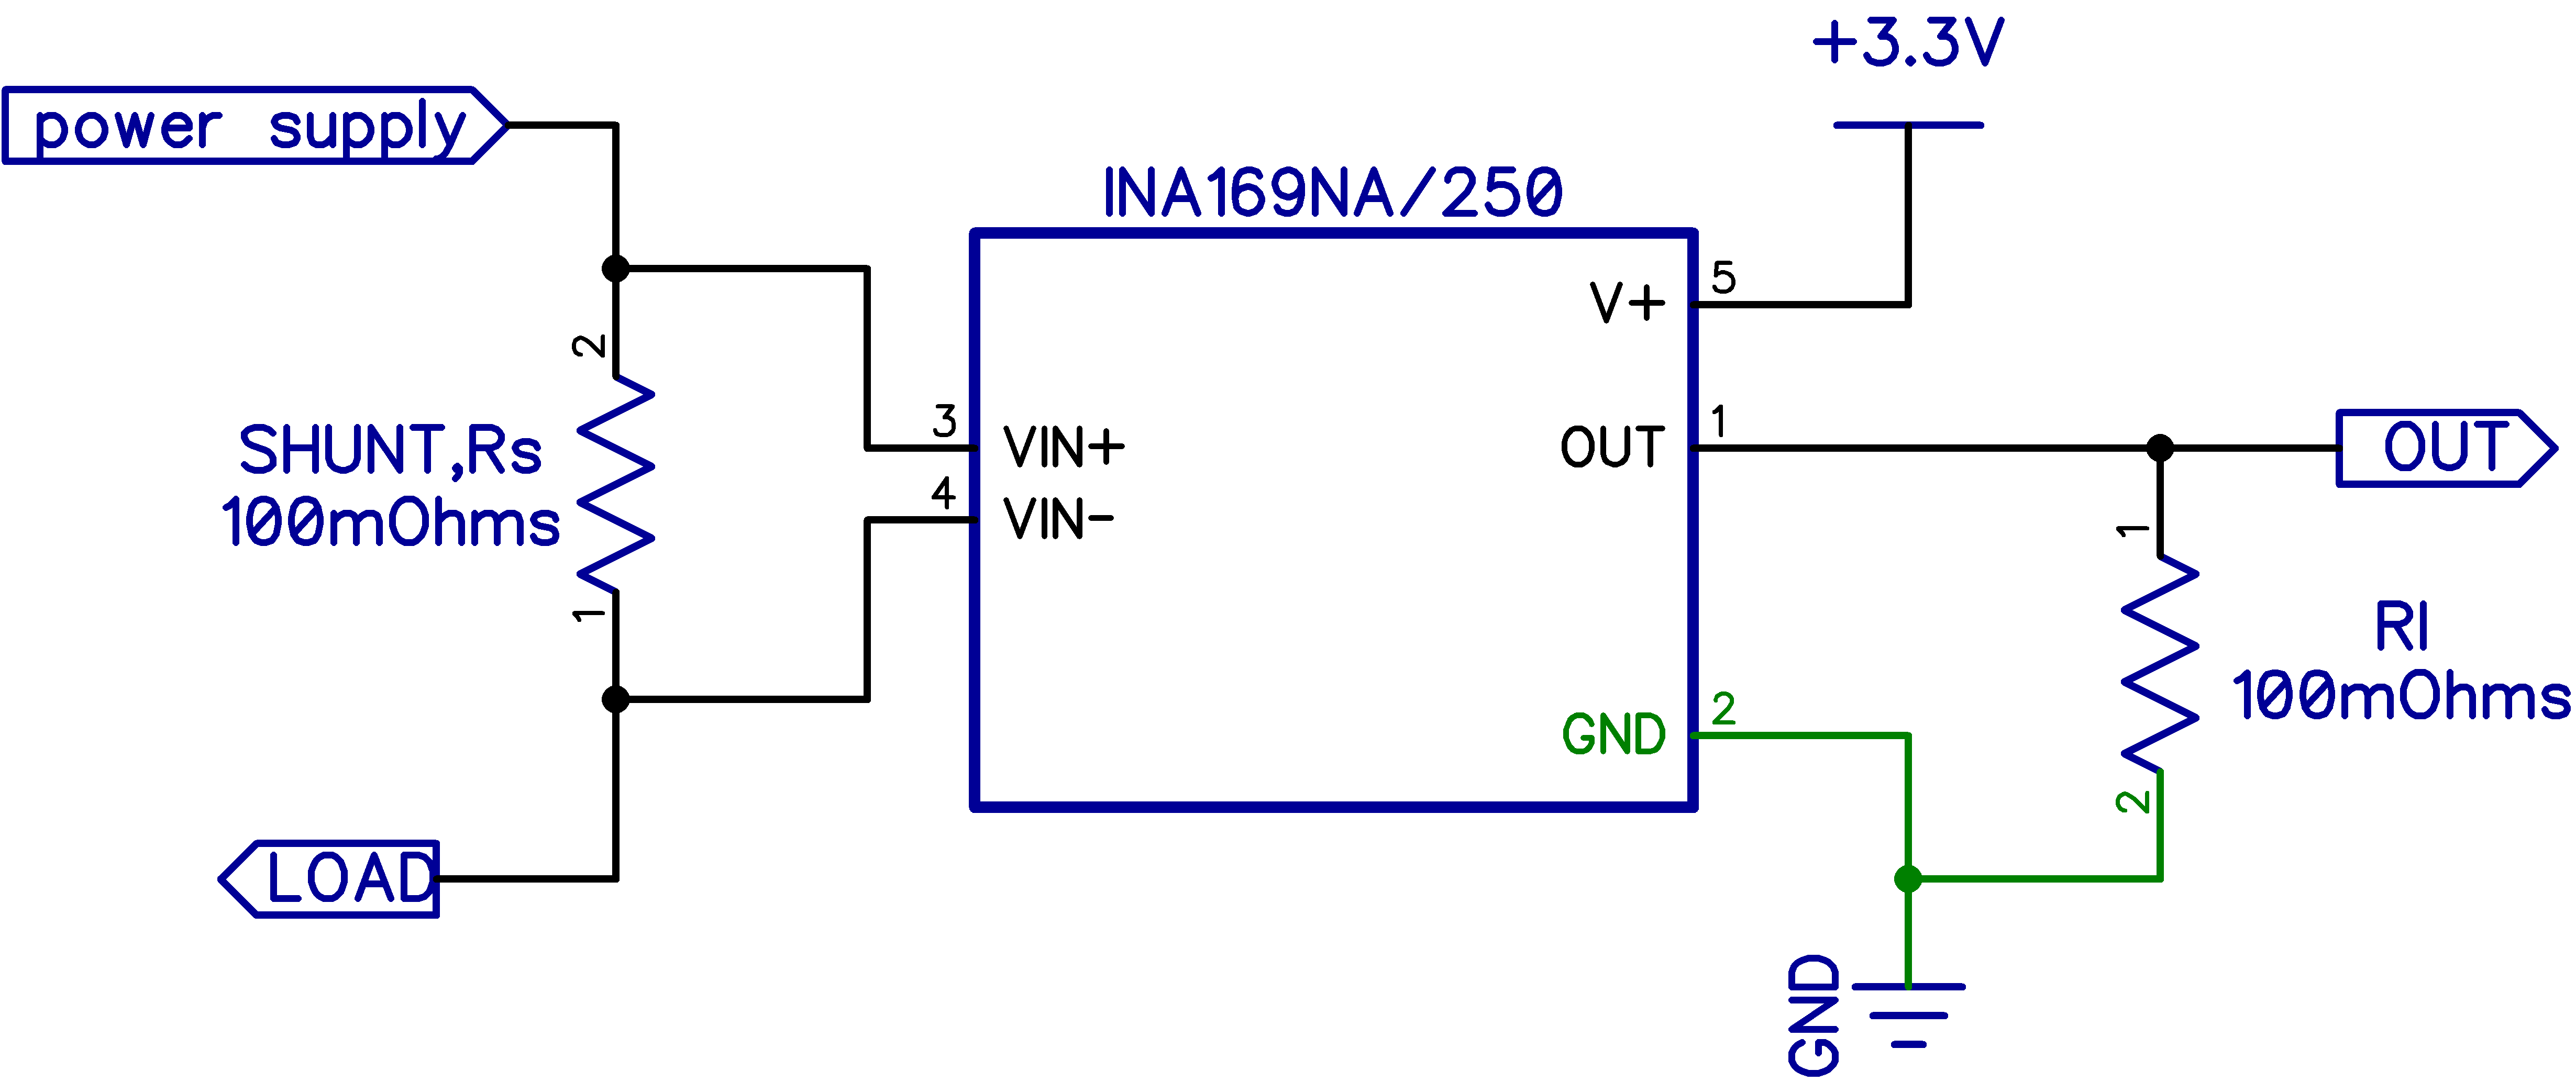
\includegraphics[width=9cm]{obr/INAschema.png}}
\hfill
\subfigure[{Senzor INA169NA/250\cite{INAobr}}]{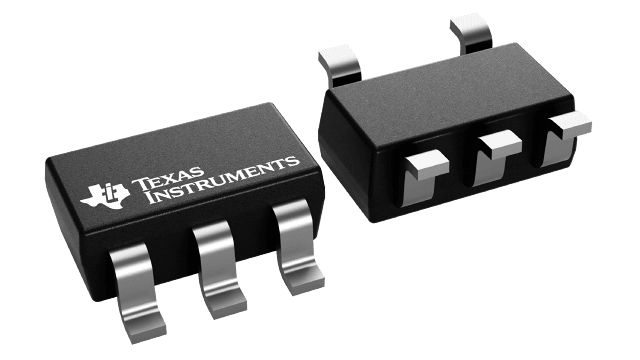
\includegraphics[width=6cm]{obr/ina.png}}
\hfill
\caption{meranie prúdu}\label{OBRAZOK 2.3}
\end{figure}


\label{Hall}
\subsubsection{meranie uhla kyvadla}

Na správne fungovanie AeroShieldu je dôležité vedieť s vysokou presnosťou merať uhol naklonenia kyvadla. Na tento účel sme si zvolili meranie uhlu bezkontaktnou formou, pomocou snímača na princípe hallovho javu. Hallov jav vieme opísať ako vznik priečneho elektrického poľa v pevnom materiáli, keď ním preteká elektrický prúd a tento materiál je umiestnený v magnetickom poli, ktoré je kolmé na prúd\cite{Hall}. Toto elektrické pole resp. vznik elektrického potenciálu vieme detegovať a na základe jeho zmeny vieme určit rotáciu kyvadla. V kyvadle je na konci horizontálneho ramena umiestnený špeciálny magnet kruhového tvaru ktorý je polarizovaný naprieč prierezom magnetu.

Ako senzor na meranie hallovho efektu je použitý AS5600 od výrobcu OSRAM obr.\ref{OBRAZOK 2.2}.b. Senzor má 12-bitový analógový výstup s rozlíšením 0°5'16". Toto rozlíšenie nám umožnuje s vysokou presnosťou kontrolovať naklonenie kyvadla a na základe zýskaných informácii ovplyvňovať fungovanie akčného členu sústavy. Schéma zapojenia čipu na meranie uhlu môžeme vidieť na obr.\ref{OBRAZOK 2.2}.a.


\begin{figure}[!tbh]
\hfill
\subfigure[Schéma zapojenia čipu na meranie uhlu.]{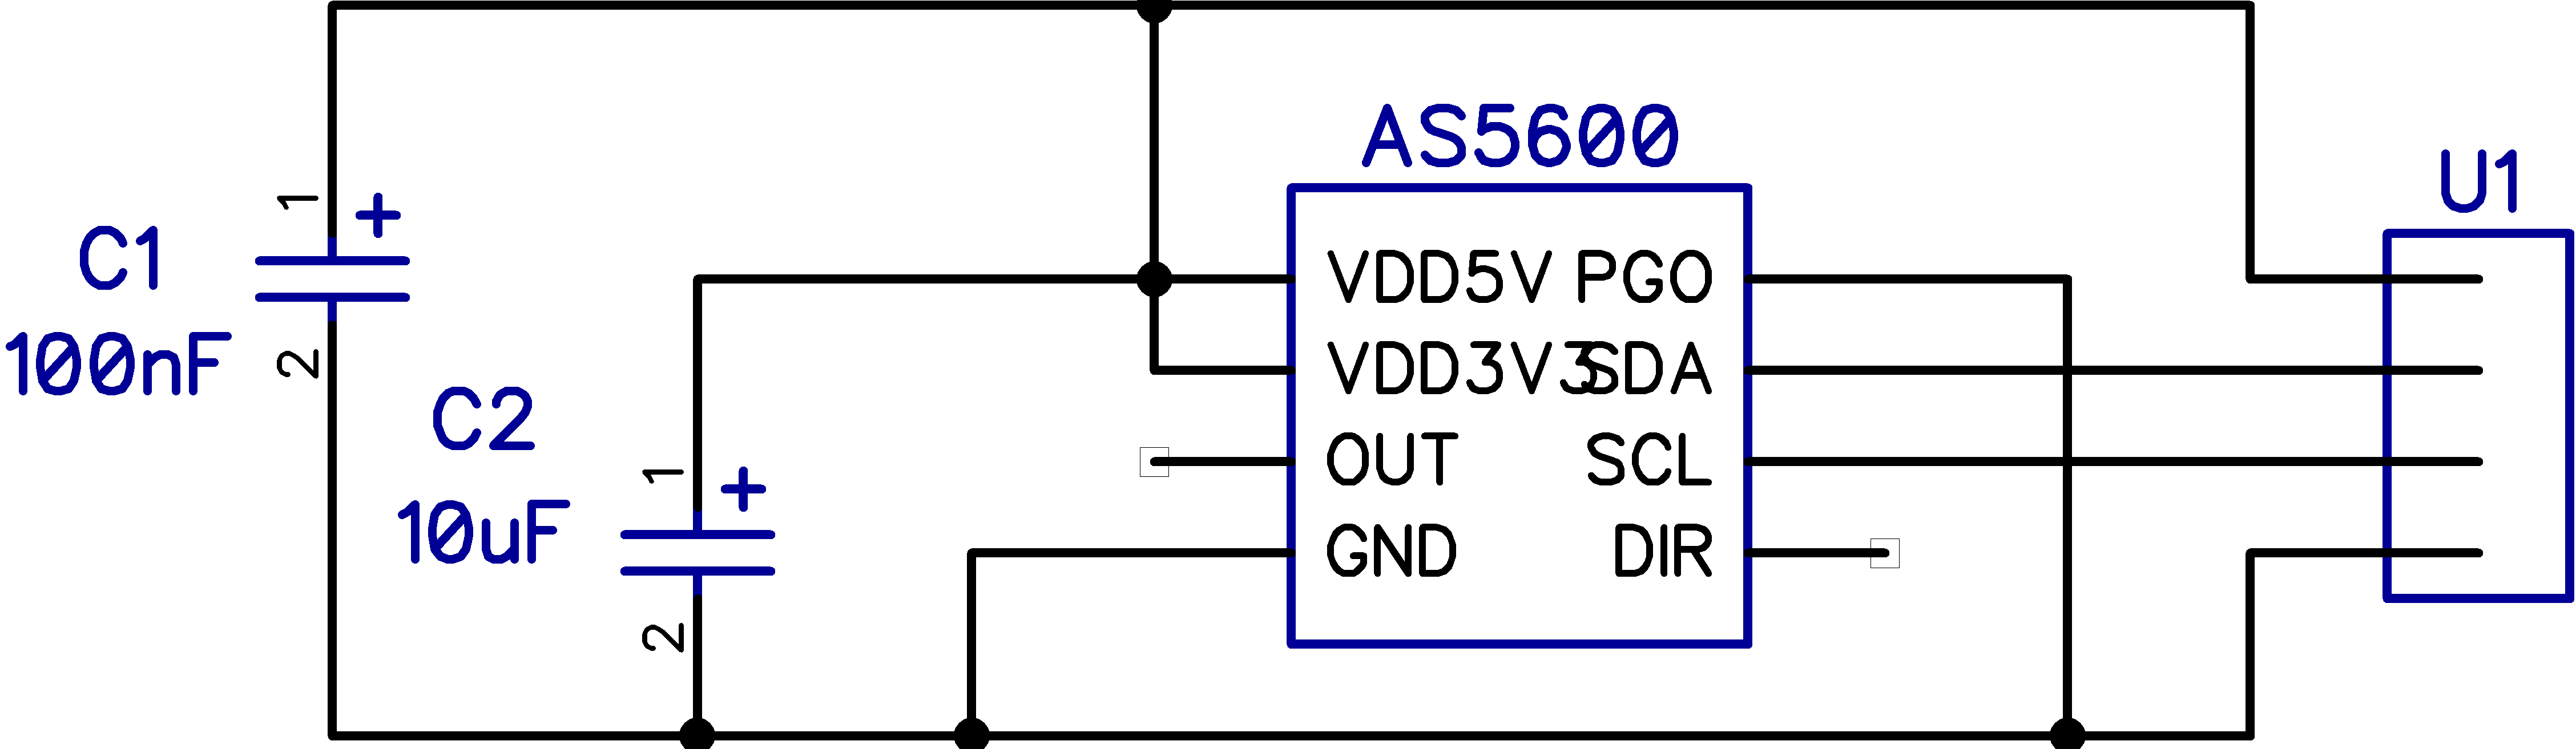
\includegraphics[width=10cm]{obr/as5600.png}}
\hfill
\subfigure[{čip AS5600\cite{As5600obr}}]{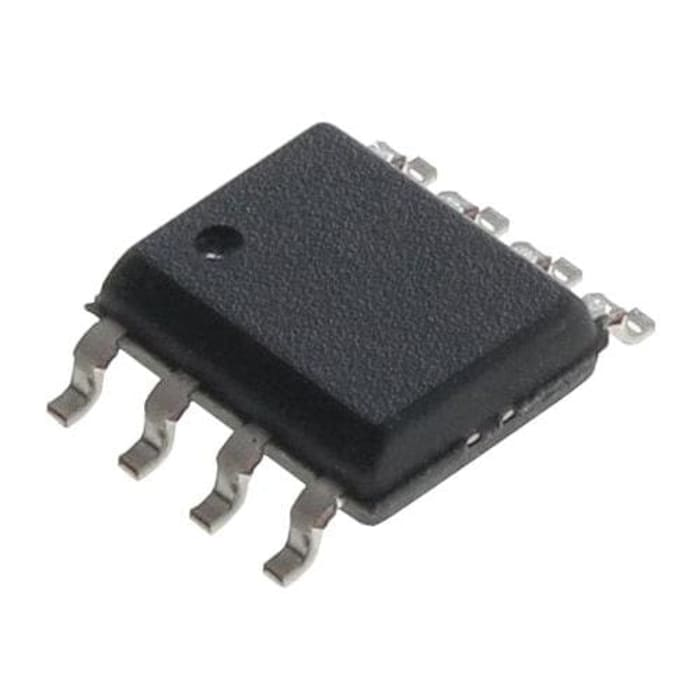
\includegraphics[width=5cm]{obr/hall.jpg}}
\hfill
\caption{meranie uhla kyvadla}\label{OBRAZOK 2.2}
\end{figure}


\subsection{Schéma zapojenia}

ZAPOJENIE HOVOR O DIPTRACE!

\subsection{Doska plošných spojov}

ZAPOJENIE HOVOR O PLOŠÁKOCH !

AJ BREAKOUT BOARD!

\section{Software}
fgdfgbh 